% !TEX encoding   = UTF8
% !TEX spellcheck = ru_RU

\documentclass[a4paper,11pt,landscape,notitlepage,oneside,openany,final]{memoir}

% !TEX encoding   = UTF8
% !TEX spellcheck = en_US


%%% Page layout %%%
\usepackage{pdflscape}
\usepackage{geometry}

%%% Mathematics %%%
\usepackage{amsthm,amsfonts,amsmath,amscd}
\usepackage{mathtools}             % Add environment 'multlined'
\usepackage{dsfont}
\usepackage{unicode-math}

%%% Encodings and fonts %%%
\usepackage{polyglossia}[2014/05/21]  % Automatically load 'fontspec'

%%% Paragraph layout %%%
\usepackage{indentfirst}
\usepackage{epigraph}
\usepackage[style=french]{csquotes}

%%% Colors %%%
\usepackage[svgnames,table,hyperref]{xcolor} %,cmyk

%%% Tables %%%
\usepackage{longtable,ltcaption}
\usepackage{multirow,makecell}     % Advanced formatting
\usepackage{tabu,tabulary}         % Automatic columns width
\usepackage{array}
\usepackage{hhline}
\usepackage{multicol}

%%% General layout %%%
\usepackage{soulutf8}              % Underlying with hyphenation
\usepackage{icomma}
\usepackage{calc}
\usepackage[normalem]{ulem}

%%% Hyper references %%%
\usepackage{hyperref}

%%% Figures %%%
\usepackage{graphicx}
\usepackage{tikz}
\usetikzlibrary{arrows,decorations.pathmorphing,backgrounds,positioning,fit,calc}
\usetikzlibrary{arrows.meta}
\usetikzlibrary{shapes,shapes.misc}
\usetikzlibrary{graphs, graphdrawing}
\usegdlibrary{trees, layered}
\usepackage{wrapfig}

%%% Lists %%%
\usepackage[inline]{enumitem}

%%% Embedded languages %%%
\usepackage[usefamily={py,sympy},rerun=always]{pythontex}

%%% Listings %%%
\usepackage{verbatim}
\usepackage{minted}
\usepackage{listings}
\lccode`\~=0\relax                 % Fix \MakeLowercase etc. with (xe|lua)latex

%%% Smart references %%%
%\usepackage{cleveref}



\usepackage{wasysym}

% !TEX encoding   = UTF8
% !TEX spellcheck = en_US


%%% Hyper references colors %%%

\definecolor{linkcolor}{rgb}{0.9,0,0}
\definecolor{citecolor}{rgb}{0,0.6,0}
\definecolor{urlcolor}{rgb}{0,0,1}



%%% Define names %%%

\newcommand*\paperOrganization{\todo{Organization}}
\newcommand*\paperOrganizationShort{\todo{OShort}}
\newcommand*\paperDepartment{\todo{Department}}
\newcommand*\paperDepartmentShort{\todo{DShort}}
\newcommand*\paperTitle{\todo{Title}}
\newcommand*\paperSubject{\todo{Subject}}
\newcommand*\paperAuthor{\todo{\textcopyright{}perto}}
\newcommand*\paperKeywords{\todo{Keywords}}
\newcommand*\paperDate{\todo{Date}}
\newcommand*\paperYear{\todo{Year}}

% !TEX encoding   = UTF8
% !TEX spellcheck = en_US


%%% Redefine names %%%

\renewcommand*\paperOrganization{Московский физико-технический институт \\
    (государственный университет)}
\renewcommand*\paperOrganizationShort{МФТИ}
\renewcommand*\paperDepartment{Факультет аэромеханики и летательной техники}
\renewcommand*\paperDepartmentShort{ФАЛТ}
\renewcommand*\paperTitle{Архитектура компьютера и язык ассемблера}
\renewcommand*\paperAuthor{\textcopyright Преподаватели}
\renewcommand*\paperKeywords{МФТИ, ФАЛТ, информатика, программирование, язык С++}
\renewcommand*\paperDate{\textit{2023--2024 уч.\,гг.}}
\renewcommand*\paperYear{2023--2024\,гг.}


\renewcommand*\paperSubject{Успеваемость (\href{\latexurl}{\TeX}нический контроль)}

% !TEX encoding   = UTF8
% !TEX spellcheck = en_US


%%% Template %%%

\DeclareRobustCommand{\todo}{\textcolor{red}}

\AtBeginDocument{%
  \setlength{\parindent}{2.5em}
}



%%% Encondings and fonts %%%

\setmainlanguage[babelshorthands=true]{russian}
\setotherlanguage{english}

\setmonofont{Source Code Pro}
\newfontfamily\cyrillicfonttt{Source Code Pro}

\defaultfontfeatures{Ligatures=TeX}  % NB! monofont settings should be before this

\setmainfont{STIX Two Text}
\newfontfamily\cyrillicfont{STIX Two Text}

\setsansfont{Source Sans 3}
\newfontfamily\cyrillicfontsf{Source Sans 3}

\setmathfont{STIX Two Math}
\newfontfamily\cyrillicfontmf{STIX Two Math}



%%% Captions %%%

\setlength{\abovecaptionskip}{0pt}
\setlength{\belowcaptionskip}{0pt}

\captionwidth{\linewidth}
\normalcaptionwidth



%%% Figures %%%

\setfloatadjustment{figure}{%
  \setlength{\abovecaptionskip}{0pt}
  \setlength{\belowcaptionskip}{0pt}
  \precaption{}
  \captionnamefont{\normalfont\normalsize}
  \captiondelim{~--- }
  \captionstyle[\centering]{\centering}
  \captiontitlefont{\normalfont\normalsize}
  \postcaption{}
}



%%% Subfigures captions %%%

\newsubfloat{figure}
\renewcommand{\thesubfigure}{\asbuk{subfigure}}
\subcaptionsize{\normalsize}
\subcaptionlabelfont{\normalfont}
\subcaptionfont{\!\!) \normalfont}  % round bracket after a letter
\subcaptionstyle{\centering}



%%% Tables %%%

\setfloatlocations{table}{!h}


%%% Hyper references settings %%%

\hypersetup{
  unicode,
  linktocpage=true,
%  linktoc=all,                % both the section and page part are links
%  pdfpagelabels=false,
  plainpages=false,
  colorlinks,
  linkcolor={linkcolor},
  citecolor={citecolor},
  urlcolor={urlcolor},
%  hidelinks,
  pdftitle={\paperTitle},
  pdfauthor={\paperAuthor},
  pdfsubject={\paperSubject},
  pdfkeywords={\paperKeywords},
  pdflang={ru},
}



%%% Lists %%%

\renewcommand{\labelitemi}{\normalfont\bfseries{--}}

%\renewcommand{\theenumi}{\alph{enumi}}
%\renewcommand{\labelenumi}{\theenumi)}

\makeatletter
\AddEnumerateCounter{\Asbuk}{\russian@Alph}{Щ}
\AddEnumerateCounter{\asbuk}{\russian@alph}{щ}
\makeatother

%\renewcommand{\theenumi}{\asbuk{enumi}}
%\renewcommand{\labelenumi}{\theenumi)}

\renewcommand{\theenumii}{\asbuk{enumii}}
\renewcommand{\labelenumii}{\theenumii)}

\renewcommand{\theenumiii}{\arabic{enumiii}}
\renewcommand{\labelenumiii}{\theenumiii)}

\setlist{%
  nosep,%
  labelindent=\parindent,leftmargin=*%
}

\newlist{enumIssue}{enumerate}{1}
\setlist[enumIssue]{label=\Asbuk*., ref=\Asbuk*}

\newlist{enumissue}{enumerate}{1}
\newlist{enumissue*}{enumerate*}{1}
\setlist[enumissue,enumissue*]{label=\textit{\asbuk*}), ref=\textit{\asbuk*}}

\newlist{itemfeature}{itemize}{1}
\setlist[itemfeature]{label=--, topsep=\medskipamount}



%%% Listings %%%

\usemintedstyle{manni}

\renewcommand{\theFancyVerbLine}{%
  \textcolor{gray}{\tiny\arabic{FancyVerbLine}}%
}

\newmintinline{c}{fontsize=\small}
\newmintinline{cpp}{fontsize=\small}
\newmintinline{gas}{fontsize=\small}
\newmintinline{text}{fontsize=\small}

\newmint[cc]{c}{fontsize=\small, escapeinside=||}
\newmint{cpp}{fontsize=\small}
\newmint{js}{fontsize=\small}
\newmint{gas}{fontsize=\small}
\newmint[txt]{text}{fontsize=\small}
\newmint{console}{fontsize=\small}
\newmint[precomment]{text}{fontsize=\footnotesize, formatcom=\color{cyan}}

\newminted{c}{linenos, fontsize=\small, numbersep=0.2em, escapeinside=||}
\newminted{cpp}{linenos, fontsize=\small, numbersep=0.2em}
\newminted{gas}{linenos, fontsize=\small, numbersep=0.2em, tabsize=2}
\newminted{text}{fontsize=\small, tabsize=2}
\newminted{console}{fontsize=\small, tabsize=2}

\newmintedfile{c}{linenos, fontsize=\small, numbersep=0.2em, stripnl}
\newmintedfile{cpp}{linenos, fontsize=\small, numbersep=0.2em}
\newmintedfile{js}{linenos, fontsize=\small, numbersep=0.2em}
\newmintedfile{gas}{linenos, fontsize=\small, numbersep=0.2em, tabsize=2}
\newmintedfile{objdump}{linenos, fontsize=\small, numbersep=0.2em, tabsize=2, escapeinside=||}
\newmintedfile{text}{fontsize=\small, tabsize=2}
\newmintedfile{console}{fontsize=\small, tabsize=2}


\newminted[precode]{text}{fontsize=\footnotesize, formatcom=\color{cyan}}



%%% General layout %%%

\DeclareRobustCommand*{\name}{\texttt}
\DeclareRobustCommand*{\code}[1]{\name{\small #1}}
\DeclareRobustCommand*{\codebf}[1]{\code{\bfseries #1}}
\DeclareRobustCommand*{\lang}[1]{\name{#1}}

\newcommand*{\comm}[1]{{\color{cyan}\ttfamily\footnotesize\itshape #1}}

\newcommand*{\styleans}[1]{\color{cyan}\underline{\color{gray!40}\ttfamily{}#1}}
\newcommand*{\showans}[1]{\phantom{#1}}
\newcommand*{\ansx}[1]{}
\newcommand*{\ansdots}[1]{\textcolor{cyan}{\ttfamily ...}}

\newcommand*{\ansfwnostar}[2]{\styleans{\makebox[#1][l]{\showans{#2}}}}
\newcommand*{\ansfwstar}[2]{\styleans{\makebox[#1][l]{\color{black}#2}}}
\newcommand*{\ansvwnostar}[1]{\styleans{\showans{#1}}}
\newcommand*{\ansvwstar}[1]{\styleans{\color{black}#1}}

\makeatletter
\newcommand*{\ansfw}{\@ifstar\ansfwstar\ansfwnostar}
\newcommand*{\ansvw}{\@ifstar\ansvwstar\ansvwnostar}
\makeatother

\newcommand*{\ArrowTo}[1]{%
  \tikz[baseline=#1]{
    \draw[white, -{Stealth[black, length=18pt, open]}] (0,0) -- (0.01,0)
  }%
}

\newcommand*{\mystyle}[1]{\textit{\ttfamily\footnotesize{}#1}}

% !TEX encoding   = UTF8
% !TEX spellcheck = en_US


%%% Template %%%

\DeclareRobustCommand{\todo}{\textcolor{red}}

\AtBeginDocument{%
  \setlength{\parindent}{2.5em}
}



%%% Encondings and fonts %%%

\setmainlanguage[babelshorthands=true]{russian}
\setotherlanguage{english}

\setmonofont{Source Code Pro}
\newfontfamily\cyrillicfonttt{Source Code Pro}

\defaultfontfeatures{Ligatures=TeX}  % NB! monofont settings should be before this

\setmainfont{STIX Two Text}
\newfontfamily\cyrillicfont{STIX Two Text}

\setsansfont{Source Sans 3}
\newfontfamily\cyrillicfontsf{Source Sans 3}

\setmathfont{STIX Two Math}
\newfontfamily\cyrillicfontmf{STIX Two Math}



%%% Captions %%%

\setlength{\abovecaptionskip}{0pt}
\setlength{\belowcaptionskip}{0pt}

\captionwidth{\linewidth}
\normalcaptionwidth



%%% Figures %%%

\setfloatadjustment{figure}{%
  \setlength{\abovecaptionskip}{0pt}
  \setlength{\belowcaptionskip}{0pt}
  \precaption{}
  \captionnamefont{\normalfont\normalsize}
  \captiondelim{~--- }
  \captionstyle[\centering]{\centering}
  \captiontitlefont{\normalfont\normalsize}
  \postcaption{}
}



%%% Subfigures captions %%%

\newsubfloat{figure}
\renewcommand{\thesubfigure}{\asbuk{subfigure}}
\subcaptionsize{\normalsize}
\subcaptionlabelfont{\normalfont}
\subcaptionfont{\!\!) \normalfont}  % round bracket after a letter
\subcaptionstyle{\centering}



%%% Tables %%%

\setfloatlocations{table}{!h}


%%% Hyper references settings %%%

\hypersetup{
  unicode,
  linktocpage=true,
%  linktoc=all,                % both the section and page part are links
%  pdfpagelabels=false,
  plainpages=false,
  colorlinks,
  linkcolor={linkcolor},
  citecolor={citecolor},
  urlcolor={urlcolor},
%  hidelinks,
  pdftitle={\paperTitle},
  pdfauthor={\paperAuthor},
  pdfsubject={\paperSubject},
  pdfkeywords={\paperKeywords},
  pdflang={ru},
}



%%% Lists %%%

\renewcommand{\labelitemi}{\normalfont\bfseries{--}}

%\renewcommand{\theenumi}{\alph{enumi}}
%\renewcommand{\labelenumi}{\theenumi)}

\makeatletter
\AddEnumerateCounter{\Asbuk}{\russian@Alph}{Щ}
\AddEnumerateCounter{\asbuk}{\russian@alph}{щ}
\makeatother

%\renewcommand{\theenumi}{\asbuk{enumi}}
%\renewcommand{\labelenumi}{\theenumi)}

\renewcommand{\theenumii}{\asbuk{enumii}}
\renewcommand{\labelenumii}{\theenumii)}

\renewcommand{\theenumiii}{\arabic{enumiii}}
\renewcommand{\labelenumiii}{\theenumiii)}

\setlist{%
  nosep,%
  labelindent=\parindent,leftmargin=*%
}

\newlist{enumIssue}{enumerate}{1}
\setlist[enumIssue]{label=\Asbuk*., ref=\Asbuk*}

\newlist{enumissue}{enumerate}{1}
\newlist{enumissue*}{enumerate*}{1}
\setlist[enumissue,enumissue*]{label=\textit{\asbuk*}), ref=\textit{\asbuk*}}

\newlist{itemfeature}{itemize}{1}
\setlist[itemfeature]{label=--, topsep=\medskipamount}



%%% Listings %%%

\usemintedstyle{manni}

\renewcommand{\theFancyVerbLine}{%
  \textcolor{gray}{\tiny\arabic{FancyVerbLine}}%
}

\newmintinline{c}{fontsize=\small}
\newmintinline{cpp}{fontsize=\small}
\newmintinline{gas}{fontsize=\small}
\newmintinline{text}{fontsize=\small}

\newmint[cc]{c}{fontsize=\small, escapeinside=||}
\newmint{cpp}{fontsize=\small}
\newmint{js}{fontsize=\small}
\newmint{gas}{fontsize=\small}
\newmint[txt]{text}{fontsize=\small}
\newmint{console}{fontsize=\small}
\newmint[precomment]{text}{fontsize=\footnotesize, formatcom=\color{cyan}}

\newminted{c}{linenos, fontsize=\small, numbersep=0.2em, escapeinside=||}
\newminted{cpp}{linenos, fontsize=\small, numbersep=0.2em}
\newminted{gas}{linenos, fontsize=\small, numbersep=0.2em, tabsize=2}
\newminted{text}{fontsize=\small, tabsize=2}
\newminted{console}{fontsize=\small, tabsize=2}

\newmintedfile{c}{linenos, fontsize=\small, numbersep=0.2em, stripnl}
\newmintedfile{cpp}{linenos, fontsize=\small, numbersep=0.2em}
\newmintedfile{js}{linenos, fontsize=\small, numbersep=0.2em}
\newmintedfile{gas}{linenos, fontsize=\small, numbersep=0.2em, tabsize=2}
\newmintedfile{objdump}{linenos, fontsize=\small, numbersep=0.2em, tabsize=2, escapeinside=||}
\newmintedfile{text}{fontsize=\small, tabsize=2}
\newmintedfile{console}{fontsize=\small, tabsize=2}


\newminted[precode]{text}{fontsize=\footnotesize, formatcom=\color{cyan}}



%%% General layout %%%

\DeclareRobustCommand*{\name}{\texttt}
\DeclareRobustCommand*{\code}[1]{\name{\small #1}}
\DeclareRobustCommand*{\codebf}[1]{\code{\bfseries #1}}
\DeclareRobustCommand*{\lang}[1]{\name{#1}}

\newcommand*{\comm}[1]{{\color{cyan}\ttfamily\footnotesize\itshape #1}}

\newcommand*{\styleans}[1]{\color{cyan}\underline{\color{gray!40}\ttfamily{}#1}}
\newcommand*{\showans}[1]{\phantom{#1}}
\newcommand*{\ansx}[1]{}
\newcommand*{\ansdots}[1]{\textcolor{cyan}{\ttfamily ...}}

\newcommand*{\ansfwnostar}[2]{\styleans{\makebox[#1][l]{\showans{#2}}}}
\newcommand*{\ansfwstar}[2]{\styleans{\makebox[#1][l]{\color{black}#2}}}
\newcommand*{\ansvwnostar}[1]{\styleans{\showans{#1}}}
\newcommand*{\ansvwstar}[1]{\styleans{\color{black}#1}}

\makeatletter
\newcommand*{\ansfw}{\@ifstar\ansfwstar\ansfwnostar}
\newcommand*{\ansvw}{\@ifstar\ansvwstar\ansvwnostar}
\makeatother

\newcommand*{\ArrowTo}[1]{%
  \tikz[baseline=#1]{
    \draw[white, -{Stealth[black, length=18pt, open]}] (0,0) -- (0.01,0)
  }%
}

\newcommand*{\mystyle}[1]{\textit{\ttfamily\footnotesize{}#1}}




\begin{document}

% !TEX encoding   = UTF8
% !TEX spellcheck = ru_RU

\thispagestyle{empty}%
\begin{center}%
  \paperOrganization
\end{center}%
%
\vspace{0pt plus 6fill}%
%
\begin{center}
  
\includegraphics[width=15em]{images/falt_logo.jpg}
\end{center}
%
\vspace{0pt plus 4fill}%
%
\begin{center}%
\paperDepartment
\end{center}%
%
\vspace{0pt plus 1fill}%
%
\begin{center}%
\textbf{\Huge\paperTitle}

\vspace{0pt plus 2fill}%
\textit{\large \paperSubject}

\vspace{0pt plus 4fill}%
\textcolor{violet}{\itshape\today}

\vspace{0pt plus 4fill}%
{Жуковский, \paperDate}
\end{center}



\newcommand*{\Hi}{\rule{0pt}{13pt}}
\newcommand*{\darkrow}{\rowcolor{black!5}}

\newcommand{\tabheaderitem}[2]{\multicolumn{1}{#1}{\multirow{2}{*}{#2}}}

\newcommand*{\task}[1]{\makebox[3.0cm]{задание №\,#1\Hi}}

\newcommand*{\groupmark}[1]{\textit{группа \textbf{#1}}}
\newcommand*{\groupsection}[1]{\AbstractSection{Группа №\,\textbf{#1}}}

\newcommand*{\pd}{\text{\(+\)\hspace{-3pt}.}}
\newcommand*{\md}{\text{\(-\)\hspace{-3pt}.}}

\newcommand*{\deadline}[1]{\textit{\bfseries\color{DarkRed!60}#1}}
\newcommand*{\notabene}[1]{\textit{\bfseries\color{DarkRed!70}#1}}


\clearpage
\noindent
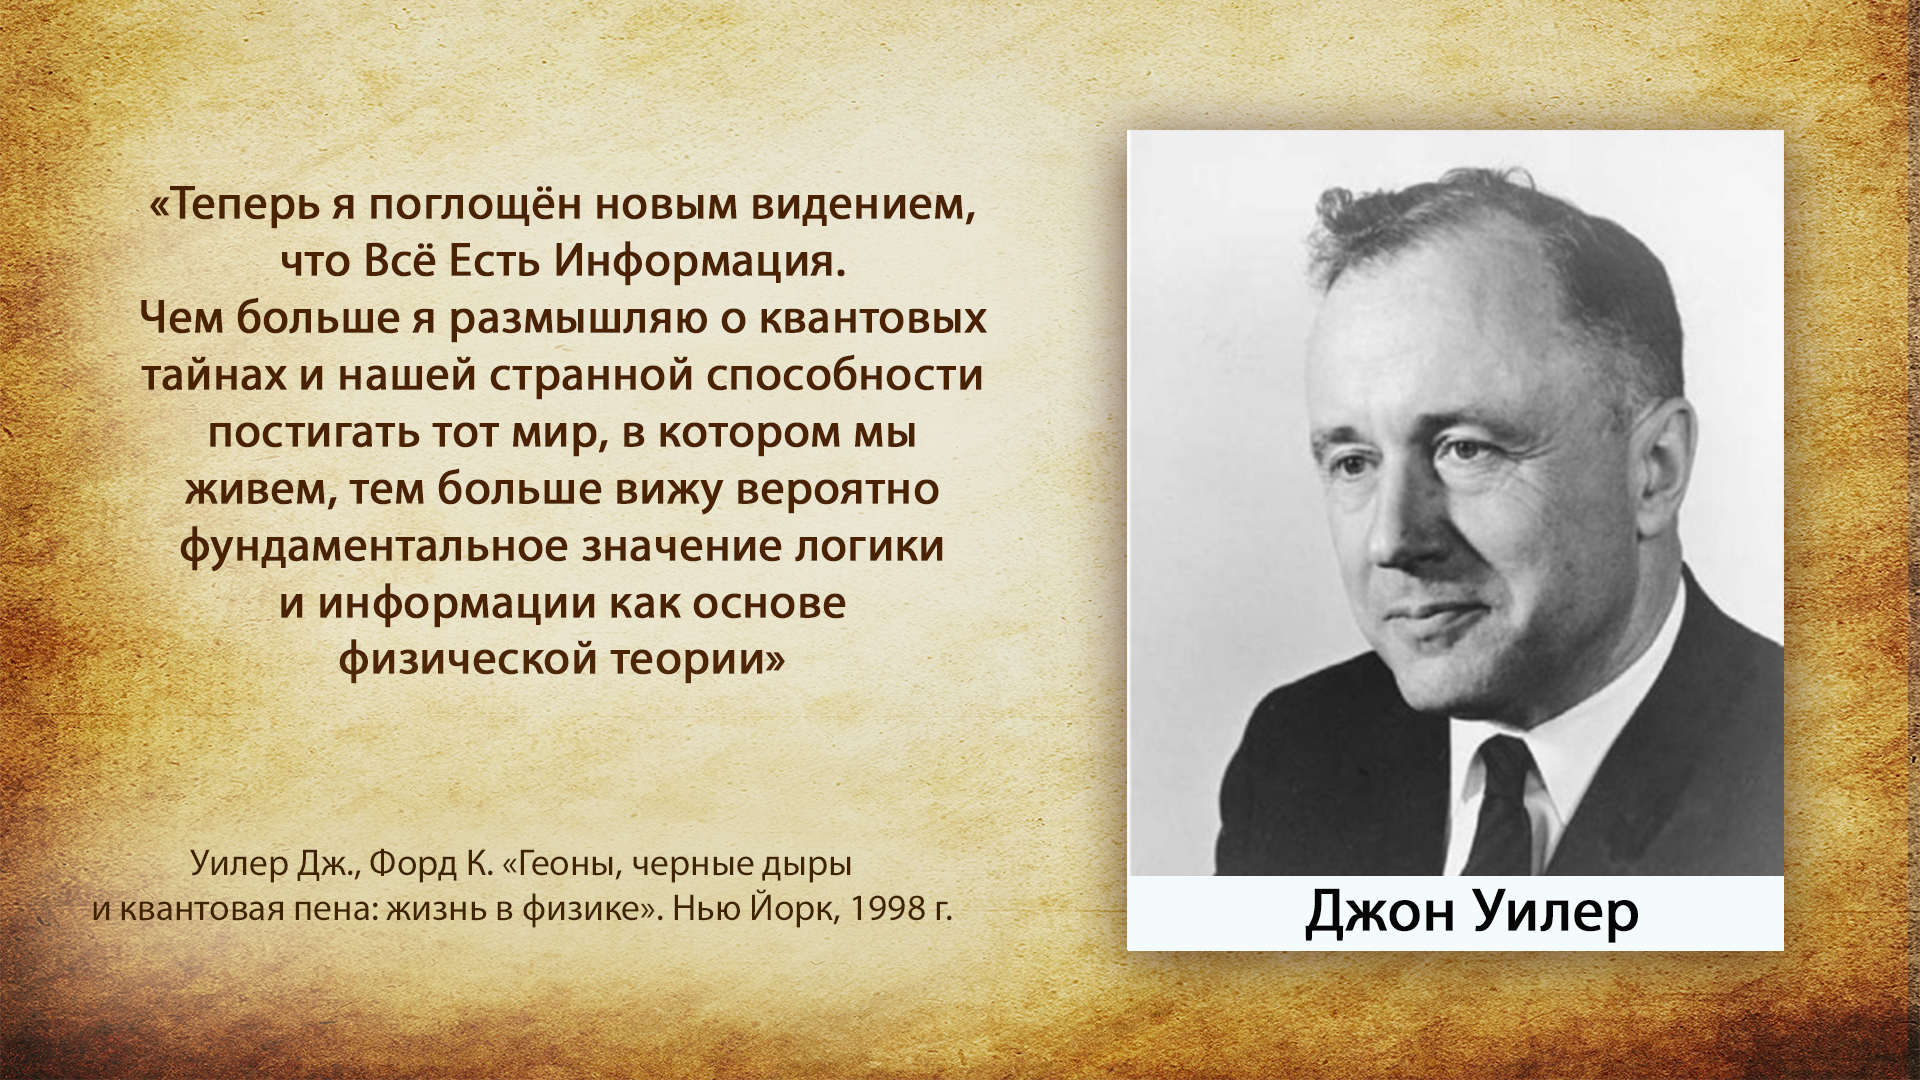
\includegraphics[width=\textwidth]{images/Джон-Уилер_RU.jpg}


\clearpage
\renewcommand{\rightmark}{Задания}
Выполняя каждое задание, используйте систему контроля версий \git{}, где это уместно. Следите за~оформлением кода, выбирайте подходящие имена переменным и функциям. Тщательно готовьте тесты. Не~перекладывайте работу разработчика на~плечи проверяющего. Это поможет и вам самим убедиться в~работоспособности кода после внесённых изменений. Задавайте вопросы на~семинарах.

\textbf{NB!} Данные задания "--- это только повод для~беседы. В~процессе сдачи могут быть заданы дополнительные вопросы и подзадачи.



%%=======================
\subsection{Задание №\,1}
%%=======================
\textbf{Срок сдачи}: не~позднее \deadline{17~марта}.


%%===========================
\paragraph{Логические схемы.}
%%===========================
Используя материал осеннего семестра (код в~папке \code{asm-seminars}), напишите программу на~языке \lang{C++}, которая будет моделировать работу и рисовать на~экране одну из~следующих логических схем:
\begin{enumissue}
    \item 4-х разрядный декодер;
    \item 4-х разрядная схема сдвига;
    \item 4-х разрядный компаратор;
    \item 4-х разрядный полный сумматор;
    \item\hard 4-х разрядный регистр на~основе D-триггеров.
\end{enumissue}

\smallskip\noindent
Обеспечить ввод входных и вывод выходных сигналов (консоль, файл или GUI), а также перерисовку схемы при~изменении входных сигналов.

\smallskip\noindent
\emph{Совет}: применяйте наследование и при~необходимости вносите правки в~базовую часть кода.


%%============================
\paragraph{Конечные автоматы.}
%%============================
Постройте конечный автомат, который получает на~вход двоичную запись натурального числа~\(x\), начиная с~младшего разряда, и выводит двоичную запись числа:
\begin{enumissue}
    \item \(x + 3\);
    \item \(3\cdot x\);
    \item \(3x + 2\);
    \item \(x\cdot \left( x\mod 3 \right)\).
\end{enumissue}


%%==========================
\paragraph{Машины Тьюринга.}
%%==========================
Обозначим как \(N_0\) множество всех неотрицательных чисел. Опишите машины Тьюринга, которые реализуют:
\begin{enumerate}
    \item\label{task:addinuni} Сложение двух чисел из~\(N_0\), данных в~двоичной системе счисления.

    \item Умножение двух чисел из~множества~\(N_0\), записанных на~ленте в~виде последовательности единиц, а именно:
    \[
        0\rightarrow 0, 1\rightarrow 01, 2\rightarrow 011, 3\rightarrow 0111, 4\rightarrow 01111, \ldots
    \]
    Назовём эту запись \emph{единичной записью} числа. Числа записаны на~ленте подряд.
\end{enumerate}


%%============================
\paragraph{Алгорифмы Маркова.}
%%============================
Записать алгорифмы Маркова, которые реализуют:
\begin{enumerate}
    \item см. машину Тьюринга \ref{task:addinuni}.
    \item Удвоение числа заданного:
    \begin{enumissue}
        \item в~виде единичной записи,
        \item в~двоичной системе счисления.
    \end{enumissue}
\end{enumerate}

%%=======================
\paragraph{Представление}
%%=======================
данных в~ЭВМ и трансляция основных конструкций языка~\lang{C} на~язык ассемблера.



%%=======================
\subsection{Задание №\,2}
%%=======================
\textbf{Срок сдачи}: не~позднее \deadline{12 мая}. %% \todo{\(\chi\chi\)}


%%=========================================================
\paragraph{Взаимодействие \lang{C/C++} и языка ассемблера.}
%%=========================================================
Дан текст (последовательность символов), содержащий не~более~100 элементов. Признаком конца текста считается символ с~кодом \code{'\backslash 0'}. Требуется:
\begin{itemize}
    \item ввести текст с~клавиатуры и записать его в~память ЭВМ;
    \item определить, обладает ли этот текст заданным свойством, указанным в~вашем варианте задания;
    \item преобразовать текст по~\emph{правилу\,1} вашего задания, если он обладает заданным свойством, и по~\emph{правилу 2} в~противном случае;
    \item вывести на~экран исходный и преобразованный тексты, а также номер и формулировку применённого правила.
\end{itemize}


%%================================
\paragraph{Требования к программе}
%%================================
\begin{enumerate}
    \item Ввод и вывод, выделение памяти, тестовая оснастка и логика выбора действий реализуются на~языке \lang{C/C++}.
    \item Действия: проверка свойства, применение правила~№\,1 и правила~№\,2 преобразования текста, "--- реализуются на~языке ассемблера для~архитектуры \name{Intel}~\name{x86\_64} в~синтаксисе~\name{AT\&T}. Каждое действие следует разместить в~отдельном модуле (файле). Реализация действия может состоять из~нескольких функций (процедур). Формулировки свойства текста и правил его преобразования для~вашего варианта следует разместить в~комментариях соответствующих модулей (в~начале файла).
    \item Вывод исходного текста должен быть выполнен сразу после ввода, до~анализа и преобразования.
    \item Вывод преобразованного текста должен быть выполнен только после завершения преобразования.
    \item Программа должна сохранять работоспособность при~любых входных данных.
    \item Необходимо разработать <<тестовую оснастку>> для~выполнения автоматического тестирования.
\end{enumerate}


%%==================
\paragraph{Варианты}
%%==================
\notabene{выдаются преподавателем.}
%%=========================
\paragraph{Свойство текста}
%%=========================
\notabene{(пример)}
\begin{enumerate}
    \item Текст оканчивается заглавной латинской буквой, которая больше не~встречается в~тексте.
    \item \ldots
\end{enumerate}


%%======================
\paragraph{Правило №\,1}
%%======================
\notabene{(пример)}
\begin{enumerate}
    \item Заменить каждую заглавную латинскую букву следующей по~алфавиту (\(A\rightarrow B\), \(B\rightarrow C\), \ldots, \(Z\rightarrow A\)).
    \item \ldots
\end{enumerate}


%%======================
\paragraph{Правило №\,2}
%%======================
\notabene{(пример)}
\begin{enumerate}
    \item Перенести в~начало текста все входящие в~него цифры с~сохранением порядка их следования.
    \item \ldots
\end{enumerate}



\newenvironment{results}[1][0pt]{
    \phantom{top of the page}
    \vspace{0pt plus 1fill}

    \noindent\hspace{#1}
    \begin{minipage}{\dimexpr\textwidth-#1\relax}
}{
    \end{minipage}

    \vspace{0pt plus 1fill}
    \phantom{bottom of the page}
}


\clearpage
\renewcommand{\rightmark}{Учебный план}
\begin{results}
    \input{data/curricula}
\end{results}


\clearpage
\renewcommand{\rightmark}{}
\begin{pycode}
import parse
import pathlib

import google_serve as gs


parse.set_rubicon(0.7)
datadir = pathlib.Path("data")
gc = gs.get_sheet(datadir/"token.json")
tabs = parse.read_json(datadir/"google_sheet.json")
for url in tabs["urls"]:
    title, table = parse.read_table(gc, url)
    print(rf"\groupsection{{{title}}}")
    print(rf"\renewcommand{{\rightmark}}{{\groupmark{{{title}}}}}")
    print("")
    print(r"\begin{results}")
    parse.print_main(table)
    print(r"\end{results}")
    print("\n\n\n")
    print(r"\clearpage")
\end{pycode}

\end{document}
